\part{Contribution}
\label{chap:deuxiemme}

\chapter{Reconnaissance de panneaux routiers à base de deep Learning}

\section{Introduction}

Cette partie sera consacrée pour la reconnaissance basée sur les réseaux de neurones profonds de type convolutionnel (CNN). Le choix de ce type de classifieur est justifié par les nombreux avantages qu’il offre par rapport aux autres techniques de classification. Ces réseaux sont une forme particulière du réseau neuronal multicouche.\\
Dans ce qui reste de ce chapitre, nous présentons tt d’abord le domaine du « deep learning »,ensuite, nous discuterons l’utilisation des réseaux de neurones convolutionnels pour les applications de classification et bien sûr par rapport à la classification des panneaux de signalisation routière, et à la fin nous entamerons la partie expérimentale de plus des différentes architectures implémentées, résultats obtenues et l’interprétation de ces deniers.

\section{Deep Learning}

On a vu dans le chapitre précédent de ce travail des généralités sur les méthodes d’apprentissage automatique (Machine Learning) et qu’il y a deux types de ces derniers: supervisé et non-supervisé, d’un autres côté, il y a aussi les méthodes d'apprentissage semi-supervisées qui se situent entre les deux types mentionnés.\\
Ces méthodes d'apprentissage sont utilisées lorsqu'une grande quantité de données d'entrée est disponible et que seules certaines données sont étiquetées. Un bon exemple est une archive de photos où seules certaines images sont étiquetées et la majorité ne le sont pas.\\
Bien que ces algorithmes d'apprentissage automatique existent depuis longtemps, la possibilité d'appliquer automatiquement des calculs mathématiques complexes à des données de grandes dimensions est un développement récent.\\
Le terme "Deep Learning" a été introduit pour la première fois à l’apprentissage automatique (ML) par Dechter (1986) \cite{45}, et aux réseaux neuronaux artificiels par Aizenberg et al (2000) \cite{46}.

\subsection{Pourquoi deep Learning ? }

Même si leurs origines remontent aux années 90 , c’est au début des années 2010 avec les travaux de Geoffrey Hinton, que les algorithmes de Deep Learning ont commencé à démontrer leurs efficacité.En effet, la puissance accrue des ordinateurs d’aujourd’hui, en termes de vitesse et de mémoire ainsi que l'apparition du "Big Data", a aidé les techniques d’apprentissage automatique à s’évoluer pour apprendre à partir d’un vaste corpus de données de formation. \\
La différence entre le Deep Learning et les algorithmes d’apprentissage automatiques, c’est l’habilité d’adaptation, de plus quand le volume de données fourni est grand,les performances du Deep Learning sont meilleurs, les modèles de Deep Learning n’ont pas de  limitations (théoriquement) et ils arrivent même à dépasser la performance humaine dans certains domaines comme la classification  et la reconnaissance d’images.(Figure- \ref{fig:vol}).Un autre volet,c'est que lors de l'analyse complexe,les algorithmes d’apprentissage automatique font l'extraction des caractéristiques essentielles du traitement manuellement alors que le Deep Learning le fait de manière automatique par l'algorithme. \cite{47}

\begin{figure}[h]
      \centering
      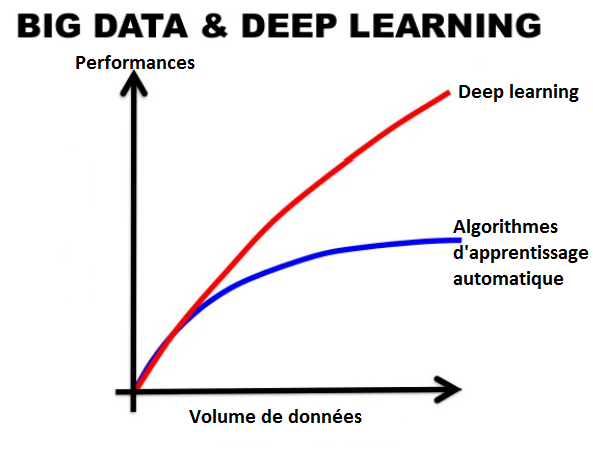
\includegraphics[width=6cm,height=4cm]{images/cnc.png}
      \caption{Différence de performance entre le Deep Learning et la plupart des algorithmes d'apprentissage automatique en fonction du volume de données}
    \label{fig:vol}
\end{figure}

En général, Le deep Learning offre trois avantages clés:
\begin{enumerate}
    \item Simplicité : les réseaux profonds offrent des blocs d'architecture de base, des couches de réseau, qui sont répétés plusieurs fois pour générer de grands réseaux au lieu d'ajustements spécifiques à un  problème ;
    \item L'évolutivité : Les modèles de deep learning sont facilement adaptables à d'énormes jeux de données. D'autres méthodes concurrentes, telles que les machines du noyau, rencontrent de graves problèmes de calcul si les jeux de données sont énormes;
    \item Transfert de domaine : Un modèle appris sur une tâche est applicable à d'autres tâches connexes.
\end{enumerate}

\subsection{Différents types de modèles }
Il existe plusieurs variantes d’architectures profondes (deep architectures) mais la majorité d’entre elles sont dérivées d’architecture originale en quelques sortes «parentales» ,et il n’est pas toujours possible de comparer les performances des architectures entre elles car ces dernières ne peuvent pas être toutes évaluées sur les même ensembles de données.\\
D’un autre côté, le Deep Learning est un domaine évolutif, de croissance rapide, de nouvelles architectures et variantes apparaissent tout le temps.\\
On trouve :
\begin{itemize}
    \item Les réseaux de neurones convolutifs(CNN): dans ce cas le problème est divisé en sous parties, et pour chaque partie, un «cluster» de neurones sera créer afin d’étudier cette portion spécifique. Par exemple, pour une image en couleur, il est possible de la diviser sur la largeur, la hauteur et la profondeur (les couleurs) ;
    \item Réseau de neurones récurrents(RNN : Recurrent Neural Network) : c'est des réseaux avec des boucles,permettant aux informations de persister,ils  sont appelés ainsi car ils exécutent la même tâche pour chaque élément d’une séquence (la sortie étant dépendante des calculs précédents) \cite{50};
   \item deep generative model : sachant que les modèles précédents essayent de prédire p(y|x) avec ‘y’ est l’étiquette et  ‘x’  l’entrée (l’image) , ce genre de modèle apprend p(x,y) et essaye de prédire et calculer le p(y|x) en utilisant la loi de Bayes\cite{49}.Il existe plusieurs modèle génétifs comme Boltzmann Machines \cite{51}, Restricted Boltzmann Machines \cite{52,53} ,Deep Belief Networks\cite{54}...etc .

\end{itemize}

\section{Réseaux de neurones convolutifs (CNN)}

Les CNN sont un excellent exemple de méthodes d’apprentissage en profondeur et ont fait l’objet des études les plus approfondies.

\subsection{Définition}
Les réseaux de neurones convolutionnels (Convolutional Neural Networks : ConvNets ) correspondent à une architecture spécifique de réseaux de neurones particulièrement adaptée au traitement des signaux 2D. Il s’agit d’une structure de réseau intégrant un mécanisme de poids partagés afin d’exploiter des propriétés locales (à court-terme et/ou spatiales).\\ L’idée principale consiste à modifier la structure d’un réseau pleinement connecté afin d’exploiter des
connexions locales : ceci conduit également à une réduction du nombre de paramètres (i.e. de poids)
du réseau.
\subsection{Pourquoi les CNN sont adaptés pour la classification des images?}
Les perceptrons multicouches (MLP) ont montré leurs efficacité comme technique d’apprentissage pour la classification de données. Ils sont en effet capables d’approximer des fonctions non–linéaires complexes afin de traiter des données de grande dimension. Dans le cadre de la classification d’images, deux approches sont possibles \cite{55}:
\begin{itemize}
    \item Extraire des caractéristiques directement des données. Classiquement, ces caractéristiques sont extraites par un algorithme choisi par l’utilisateur. Les vecteurs de caractéristiques obtenus sont ensuite présentés en entrée d’un réseau de neurones.
     \item Présenter l’image en entrée d’un réseau de neurones. L’image est alors mise sous forme d’un vecteur dont la dimension est égale au nombre de pixels de l’image.
\end{itemize}
Dans le premier cas, le réseau se contente d’effectuer une classification des vecteurs de
caractéristiques. Le point sensible (l’extraction des caractéristiques) est laissé à la discrétion de
l’utilisateur, et le choix de l’algorithme permettant l’extraction des caractéristiques est crucial.
Dans le deuxième cas, plusieurs problèmes se posent \cite{55}:
\begin{enumerate}
    \item Classiquement, les couches d’un réseau de neurones sont complètement connectées,c’est-à-dire que la valeur d’un neurone d’une couche 'n' va dépendre des valeurs de tous les neurones de la couche 'n−1'. Ainsi le nombre de connexions (et donc de poids) peut être très grand. Par exemple, pour une image de taille 15 × 15, la dimension de l’entrée d’un MLP est de 225. Si la couche cachée
comporte 100 neurones, alors le nombre de paramètres de cette couche est de 100 ×225 = 22500. Le nombre de paramètres va ainsi augmenter exponentiellement avec la
dimension de l’entrée (des images). Cette grande complexité du réseau impose d’avoir de nombreux échantillons d’apprentissage, ce qui n’est souvent pas le cas, voir impossible à réaliser. Le réseau va donc proposer une mauvaise capacité de généralisation.
    \item Un autre défaut des MLP est qu’ils sont peu ou pas invariants à des transformations de
l’entrée, ce qui arrive très souvent avec des images (légères translations, rotations ou distorsions).
    \item Enfin, les MLP ne prennent pas en compte la corrélation entre les pixels d’une image,ce qui est un élément très important pour la reconnaissance de formes.
 \end{enumerate}   
Les réseaux de neurones convolutionnels (CNN) sont une extension des MLP permettant de répondre efficacement aux principaux défauts de ces derniers. Ils sont conçus pour extraire automatiquement les caractéristiques des images d’entrée,et implémentent la notion de partage des poids permettant de réduire considérablement le
nombre de paramètres du réseau .\\
Les réseaux de neurones convolutionnels (CNN) sont maintenant un moyen standard de classification des images \cite{56}. Les modèles les plus performants pour classer des images sont les CNN, car ils se basent sur trois idées architecturales clé \cite{57}:
1) Des champs récepteurs locaux;
2) Un principe de partage des poids;
3) Des opérations de sous-échantillonnage : qui permettent de réduire la sensibilité aux
translations, ainsi que de réduire le coût du traitement

\begin{figure}[h]
      \centering
      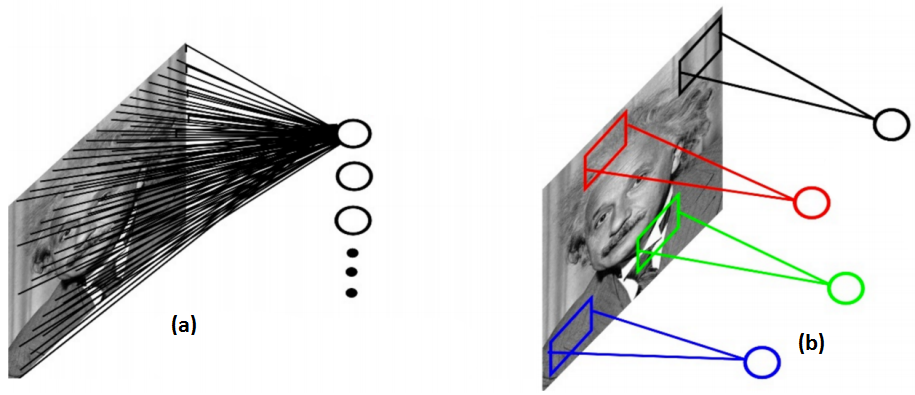
\includegraphics[width=9cm,height=4cm]{images/aysh.png}
      \caption{Illustration de la différence entre un réseau multicouche (a) et un réseau Convolutionnel}
    \label{fig:vol}
\end{figure}

\subsection{Architecture d’un réseau de neurones convolutionnel}

Les réseaux de neurones convolutionnels comportent deux parties bien distinctes (Figure- \ref{fig:archh}). En entrée, une image est fournie sous la forme d’une matrice de pixels. Elle a deux
dimensions pour une image en niveaux de gris.‎ La couleur est représentée par une troisième
dimension.\\
La première partie qui compose un réseau de neurone convolutionnel est celle qui comporte
les couches de convolutions. Cette partie fonctionne comme un extracteur de caractéristiques des
images. Une image est passée à travers une succession de filtres, ou noyaux de convolution, créant
de nouvelles images appelées cartes de convolutions. Certains filtres intermédiaires réduisent la résolution de ces cartes par une opération de sélection de maximum local ou moyenne.\\ 
Au final, les cartes de convolutions sont mises à plat et concaténées en un vecteur de caractéristiques,appelé
code CNN.

\begin{figure}[h]
      \centering
      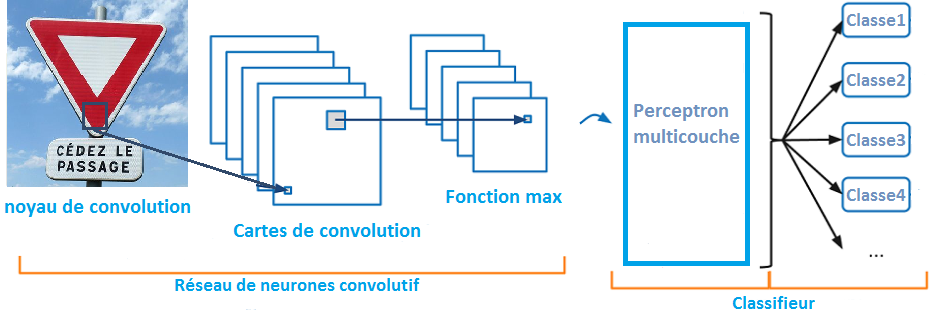
\includegraphics[width=11cm,height=4cm]{images/arch-cnn.png}
      \caption{Architecture d'un réseau de neurone convolutionnel}
    \label{fig:archh}
\end{figure}

La sortie de la partie convolutive est ensuite branché en entrée d’une deuxième partie, constituée de couches entièrement connectées (perceptron multicouche). Le rôle de cette partie est de combiner les caractéristiques du code CNN pour classer l’image. La sortie du réseau est une couche comportant un neurone par catégorie. Les valeurs numériques obtenues sont
généralement normalisées entre 0 et 1, de somme 1, pour produire une distribution de probabilité sur les catégories \cite{58}.\\
Dans un réseau CNN les couches convolutionnelles alternent avec des couches de sous-échantillonnage, qui rappellent des cellules simples et complexes dans le cortex visuel primaire.
Nous donnons ici une brève description des blocs de construction principaux).\\

{\textbf{Couche d'entrée}}\\

Tous les pixels de l’image sont éclatés en un seul vecteur, et la valeur du neurone d’entrée correspond à l’intensité du pixel associé.\\

{\textbf{Couche de convolution}}\\

Une couche convolutive est constituée de neurones qui se connectent aux sous-régions des images d'entrée ou aux sorties de la couche qui les précède. Une couche convolutionnelle apprend les caractéristiques localisées par ces régions lors de la numérisation d'une image \cite{59}.\\
Pour chaque
région, on calcule un produit scalaire des poids et de l'entrée, puis on ajoute un terme de biais.
Un ensemble de poids appliqués à une région de l'image est appelé un filtre. Le filtre se
déplace le long de l'image d'entrée verticalement et horizontalement, en répétant le même calcul
pour chaque région, c'est-à-dire en convolvant l'entrée avec le filtre. La taille du pas avec lequel le
filtre parcourt l’image s'appelle une foulée \cite{59}. La Couche de convolution donne « des cartes
d’activation » on les appelle aussi « des cartes caractéristiques ». La profondeur de ce filtre doit être la même que la profondeur de l'entrée \cite{60}\\.

{\textbf{Couche de normalisation des lots}}\\

Cette couche permet de normaliser ses entrées Xi en calculant d'abord la moyenne :\[mu _B\]  et la variance : 
 \[\sigma _B^{2}\]
 sur un mini-lot pour chaque canal d'entrée. 
Ensuite, la couche décale l'entrée d'un décalage β et l’a mis à l'échelle par un facteur γ. Les variables β et γ sont eux-mêmes des paramètres à apprendre qui sont mis à jour pendant l'apprentissage du réseau \cite{59}.\\
                \[y_i=\gamma \hat{x_i}+\beta\]


{\textbf{Couche de regroupement (pooling)}}\\

Le but de cette couche est de réduire progressivement la quantité de variables, ce qui permet un degré d’information optimal. Il existe plusieurs types de couche de regroupement : maximum,minimum, moyenne …etc.\\

{\textbf{Couche de décrochage (dropout Layer)}}\\

La couche de décrochage permet de désactiver un certain nombre de neurones, choisis d’une manière aléatoire, et qui change d’une itération d’apprentissage à une autre. 

{\textbf{Couche entièrement connectée}}\\

Comme son nom l'indique, tous les neurones d'une telle couche se connectent à tous les neurones de la couche précédente. Cette couche combine toutes les caractéristiques (informations
locales) apprises par les couches précédentes à travers l'image pour identifier les plus grands motifs.\\
La dernière couche entièrement connectée combine les fonctionnalités pour classer les images. C'est la raison pour laquelle le nombre de sortie de la dernière couche entièrement connectée du réseau est égal au nombre de classes de l'ensemble de données.\\

{\textbf{Couches de sortie}}\\

Pour les problèmes de classification, une couche softmax et ensuite une couche de classification doivent suivre la couche finale entièrement connectée. Cette couche fournie la probabilité de chaque classe.

\subsection{Réseaux convolutifs célèbres}

Plusieurs architectures dans le domaine des réseaux de convolution ont un nom , les plus courants sont :
\begin{enumerate}
    \item {\textbf{LeNet}}\\
    L'architecture LeNet est la plus connu car c'est parmis les premières applications réussies des réseaux de neurones de convolution (dans les années 1990) \cite{64},elle est principalement utilisée pour lire les codes postaux, les chiffres ...etc.
    \item {\textbf{AlexNet}}\\
    Ce type présente le premier travail qui a popularisé les réseaux de convolution dans la vision par ordinateur,développeé par Alex Krizhevsky et Ilya Sutskever et Geoff Hinton \cite{61}.Le réseau a une architecture très similaire à celle du LetNET mais plus profonde et comporte des couches convolutives superposées.\\
    \item {\textbf{ZF Net}}\\
    C'est un réseau convolutionnel de Matthew Zeiler et Rob Fergus \cite{62},c'est une amélioration pour Alexnet, en modifiant les hyperparamétres d'architecture et qui donne une meilleur précision.\\
    
    \item {\textbf{GoogLeNet}}\\
      C'est un réseau de concolution de Szegedy et al. \cite{63} de Google, sa principale contribution a été la mise au point d'un module de démarrage réduisant considérablement le nombre de paramètres dans le réseau,ainsi, il utilise le regroupement moyen au lieu de couches entièrement connectées en début du CNN,afin d'éliminer une grande quantité de paramètres.Il existe également plusieurs versions de suivi de GoogleNet,la plus récente est celle nommée \textit{Inception-V4}.   
    \item {\textbf{VGGNet}}\\
    Ce réseau convolutionnel est propre au Karen Simonyan et Andrew Aisserman \cite{65} qui présente une architecture simple basée sur Alexnet, sa contribution a été de montrer que la profondeur du réseau est un élément 
    \item {\textbf{Spatial Transformer Network}}\\
\end{enumerate}

\section{Reconnaissance de panneaux routiers basée sur les réseaux de neurones convolutifs (CNN) }

\subsection{Introduction}
Dans cette partie du chapitre on va entamer la partie expérimentale qui concerne l'implémentation de deux architectures de CNN, notamment les: VGGnet et les Spatial Transformer Network.\\
Le choix de ces deux architectures parmi celle mentionnées précédemment revient au fait que les travaux réalisés dans la littérature montrent que les « VGGnet », par rapport aux autres modèles, donnent les meilleurs résultats jusqu’à l’arrivée des modèles de « Spatial Transformer Network » en 2015 qui ont bouleversé les choses.
\subsection{Implémentations et Résultats}
\begin{enumerate}
    \item {\textbf{Chargement de données}}\\
    On a chargé deux types de données (de taille 32x32 ) à partir du GTRSB (base de données publique) :
    \begin{itemize}
        \item données réelles(avec 43 classes différentes ) ;
        \item données synthétisées(avec 43 classes différentes );
    \end{itemize}
    Ensuite, ces données subissent des sérialisations afin d’améliorer le temps de lecture de ces dernière (pickled data).Ces données sont décomposées en trois classes:
    \begin{itemize}
        \item données d'entraînement;
        \item données de test;
        \item données de validation.
    \end{itemize}
  \item {\textbf{Exploration de données}}\\
    Les données sérialisées constituent un dictionnaire de 4 paires (clé/valeur):
     \begin{itemize}
        \item features;
        \item labels;
        \item sizes;
        \item coords .
    \end{itemize}
    L'exploitation des données après traitement donne le nombre des images pour chaque classe mentionnée précédemment :
    \begin{itemize}
        \item Nombre des données d'entrainement est de 347799;
        \item Nombre des données de test est de 12630;
        \item Nombre des données de validation est de 4410;
        \item Forme d'image (32,32,3).
    \end{itemize}
    Ainsi les histogrammes suivants montrent les résultats de l'exploitation (Figure) .
    \item {\textbf{Traitement de données}}\\
    Dans cette partie, on va utilisé plusieurs étapes de traitements sur les images d'entrées qui sont déjà préparées pour aboutir à des meilleurs résultats.Les techniques principales utilisées sont :
   \begin{itemize}
        \item Shuffling;
        \item Grayscaling;
        \item Local Histogram Equalization;
        \item Normalization.
    \end{itemize}
    \item {\textbf{Conception des deux modéles utilisés: "VGGnet" et "Spatial Transformer"}}\\
     \begin{itemize}
        \item VGGnet;
        \item Spatial Tranformar Network.
        
    \end{itemize}
    \item {\textbf{Entrainement des deux modéles et Evaluation des résultats}}\\
    L'entraînement sera effectué par les deux types de données qui sont préparées dans les étapes précédentes..
     \item {\textbf{Evaluation  des modéles par les données de test}}\\
     
    \item {\textbf{Résulats et Comparaison}}\\




\end{enumerate}

\section{Conclusion}
A partir de cette partie , on a pu voir des généralités sur les modelés utilisés des réseaux de neurones convolutifs par rapport à leurs utilisation dans le domaine de classification de panneaux routiers et grâce à la partie implémentation on pu voir et interpréter les différents résultats obtenus.








